\chapter{Энергия, импульс и электромагнитное поле}

Последняя лекция начинается с исправления и заканчивается объектом, который будет стоять в правой части уравнения Эйнштейна. Этот путь не является обходным. Сначала нужно явно зафиксировать знаковое соглашение для электрического поля; затем нужно развести три различных смысла слова «импульс». Лишь после этих предварительных замечаний теорию поля можно рассматривать как обычную механику с одной степенью свободы в каждой точке пространства. После этого в рамках одного непрерывного рассуждения появляются гамильтониан, локальная плотность энергии, нётеровский импульс, электромагнитная энергия и вектор Пойнтинга.

\section{Соглашение, которое необходимо последовательно соблюдать}

Предварительные заметки должны были быть выложены для курса, но вопрос достаточно важен, чтобы разобрать его вслух. Byron заметил несогласованность не внутри обозначений курса, а между этими обозначениями и обозначениями, используемыми почти повсюду. Это профессиональный риск, когда уравнения выводятся заново: внутренне согласованное частное соглашение может отклониться от общепринятого.

Обозначим через \(\mathbf E_M\) стандартное соглашение Максвелла--Франклина, а через \(\mathbf E_L\) — соглашение, использовавшееся в предыдущих лекциях. Если использовать принятую в курсе ковариантную компоненту \(A_0\), получаем
\begin{align}
\mathbf E_M
  &= -\dot{\mathbf A}+\boldsymbol{\nabla}A_0,
&
\mathbf E_L
  &= +\dot{\mathbf A}-\boldsymbol{\nabla}A_0
   =-\mathbf E_M .
\label{eq:two-electric-conventions}
\end{align}
Во многих книгах вместо этого вводят скалярный потенциал \(\Phi=-A_0\); тогда первая формула принимает вид
\(\mathbf E_M=-\dot{\mathbf A}-\boldsymbol{\nabla}\Phi\).
Магнитное поле не меняется:
\begin{equation}
\mathbf B=\boldsymbol{\nabla}\times\mathbf A.
\label{eq:B-from-A-opening}
\end{equation}

В рационализованных единицах, где \(c=1\), стандартные уравнения Максвелла--Франклина имеют вид
\begin{align}
\boldsymbol{\nabla}\times\mathbf E_M&=-\dot{\mathbf B},
&
\boldsymbol{\nabla}\cdot\mathbf B&=0,
\nonumber\\
\boldsymbol{\nabla}\times\mathbf B&=\dot{\mathbf E}_M+\mathbf J_F,
&
\boldsymbol{\nabla}\cdot\mathbf E_M&=\rho_F .
\label{eq:maxwell-franklin}
\end{align}
Исторический выбор Бенджамина Франклина фиксирует знак заряда: в этом соглашении электрон отрицателен. Принятое в курсе соглашение также обращает обозначения источников,
\begin{equation}
\mathbf J_L=-\mathbf J_F,
\qquad
\rho_L=-\rho_F.
\label{eq:source-convention-map}
\end{equation}
Поэтому подстановка \(\mathbf E_L=-\mathbf E_M\) дает
\begin{align}
\boldsymbol{\nabla}\times\mathbf E_L&=+\dot{\mathbf B},
&
\boldsymbol{\nabla}\cdot\mathbf B&=0,
\nonumber\\
\boldsymbol{\nabla}\times\mathbf B&=-\dot{\mathbf E}_L-\mathbf J_L,
&
\boldsymbol{\nabla}\cdot\mathbf E_L&=\rho_L .
\label{eq:maxwell-course-convention}
\end{align}

\begin{figure}[H]
\centering

\includegraphics[width=\linewidth]{lecture_10_figure_01.png}
\caption{Полное сопоставление на доске между соглашениями Максвелла--Франклина и принятым в курсе.}
\par\smallskip
\textit{Кадр лекции: 00:07:10.}
\end{figure}

Ни одна измеримая величина не зависит от того, какой словарь соответствий выбран. Важно лишь сохранять последовательность, особенно когда вычисленное поле сравнивается с опубликованным экспериментальным значением. Забавность ситуации в том, что в собственной работе лектора такие прямые численные сравнения встречались настолько редко, что противоположный знак оставался незамеченным, пока на него не указала аудитория. В электромагнитном расчете далее в этой главе мы будем использовать стандартное поле \(\mathbf E\equiv\mathbf E_M\).

\section{Три разные величины, называемые импульсом}

Теперь нужно разобрать слово \emph{импульс}. Механический импульс, канонический импульс и нётеровский импульс могут совпадать в простых задачах, но это не три описания одной величины. В общей системе их численные значения могут различаться.

\subsection{Механический импульс}

Для тела полной массы \(M\) механический импульс равен
\begin{equation}
\mathbf P_{\mathrm{mech}}=M\dot{\mathbf X}_{\mathrm{cm}}.
\label{eq:mechanical-momentum}
\end{equation}
Для одной частицы \(\mathbf X_{\mathrm{cm}}\) — это просто ее положение. Для составного тела оговорка о центре масс существенна.

\begin{figure}[H]
\centering
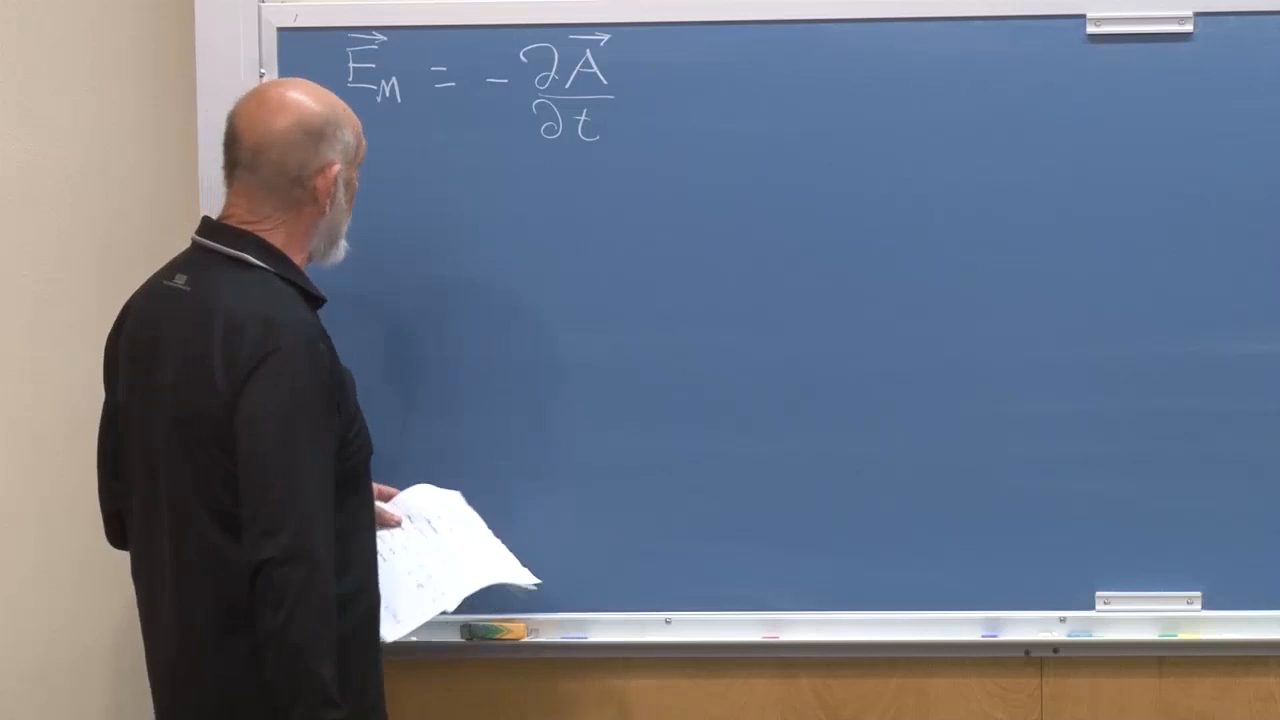
\includegraphics[width=\linewidth]{lecture_10_figure_02.png}
\caption{Механический импульс вводится как масса, умноженная на скорость центра масс.}
\par\smallskip
\textit{Кадр лекции: 00:11:15.}
\end{figure}

\subsection{Канонический импульс}

Пусть механика описывается \(L(q_i,\dot q_i)\). Канонический импульс, сопряженный с \(q_i\), равен
\begin{equation}
p_i=\frac{\partial L}{\partial\dot q_i}.
\label{eq:canonical-momentum}
\end{equation}
Для
\begin{equation}
L=\frac12 m\dot{\mathbf x}^{\,2}-V(\mathbf x),
\label{eq:simple-particle-lagrangian}
\end{equation}
отсюда получается \(\mathbf p=m\dot{\mathbf x}\), так что канонический и механический импульсы в этом случае совпадают.

\begin{figure}[H]
\centering
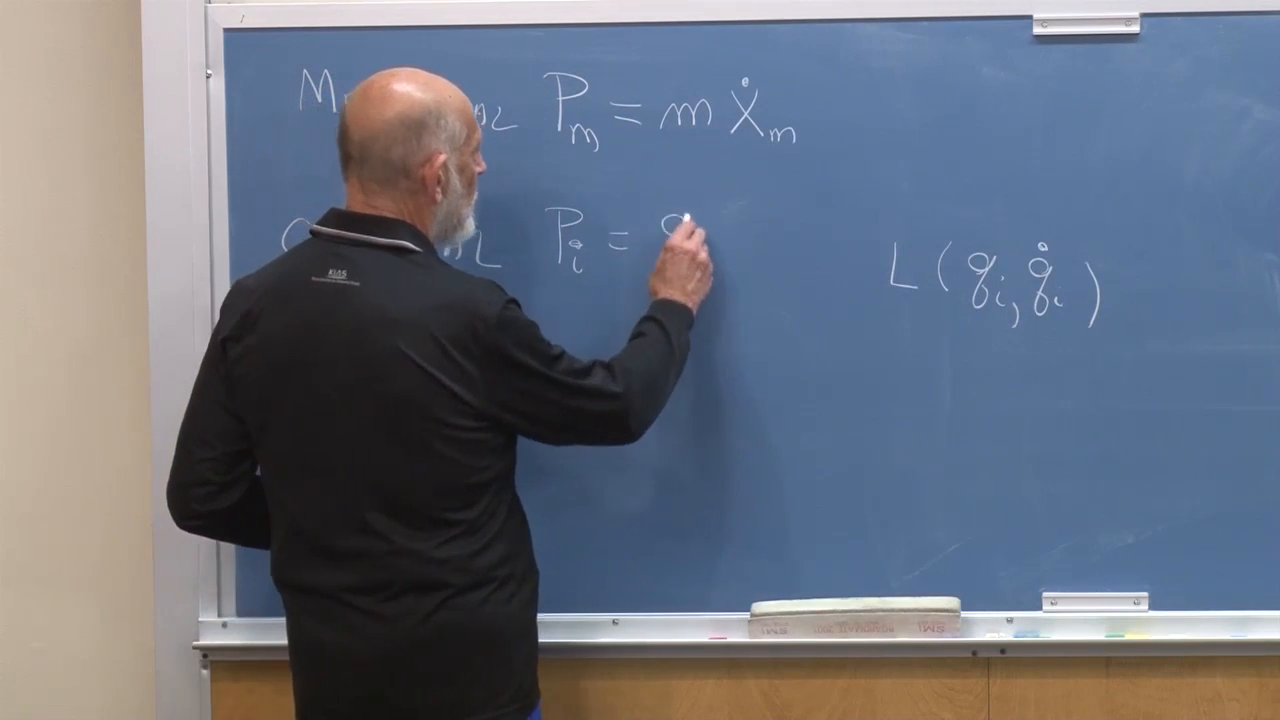
\includegraphics[width=\linewidth]{lecture_10_figure_03.png}
\caption{Механический и канонический импульсы рядом с лагранжианом простой частицы.}
\par\smallskip
\textit{Кадр лекции: 00:13:40.}
\end{figure}

Заряженная частица в магнитном поле дает удобный контрпример. При знаковом соглашении, записанном на доске,
\begin{equation}
L=\frac12m\dot{\mathbf x}^{\,2}-V(\mathbf x)
  -e\,\dot{\mathbf x}\cdot\mathbf A(\mathbf x),
\label{eq:magnetic-particle-lagrangian}
\end{equation}
и потому
\begin{equation}
p_i=m\dot x_i-eA_i.
\label{eq:magnetic-canonical-shift}
\end{equation}
Если изменить соглашение о знаке заряда или о знаке члена взаимодействия, написанный знак изменится, но вывод останется тем же: канонический импульс содержит вклад векторного потенциала и не сводится просто к \(m\dot x_i\). Уравнения Гамильтона используют каноническую переменную. Позднее можно перенести зависящий от поля член в другую часть уравнения и получить ускорение ньютоновского вида, но такая перегруппировка не меняет определения.

\begin{figure}[H]
\centering
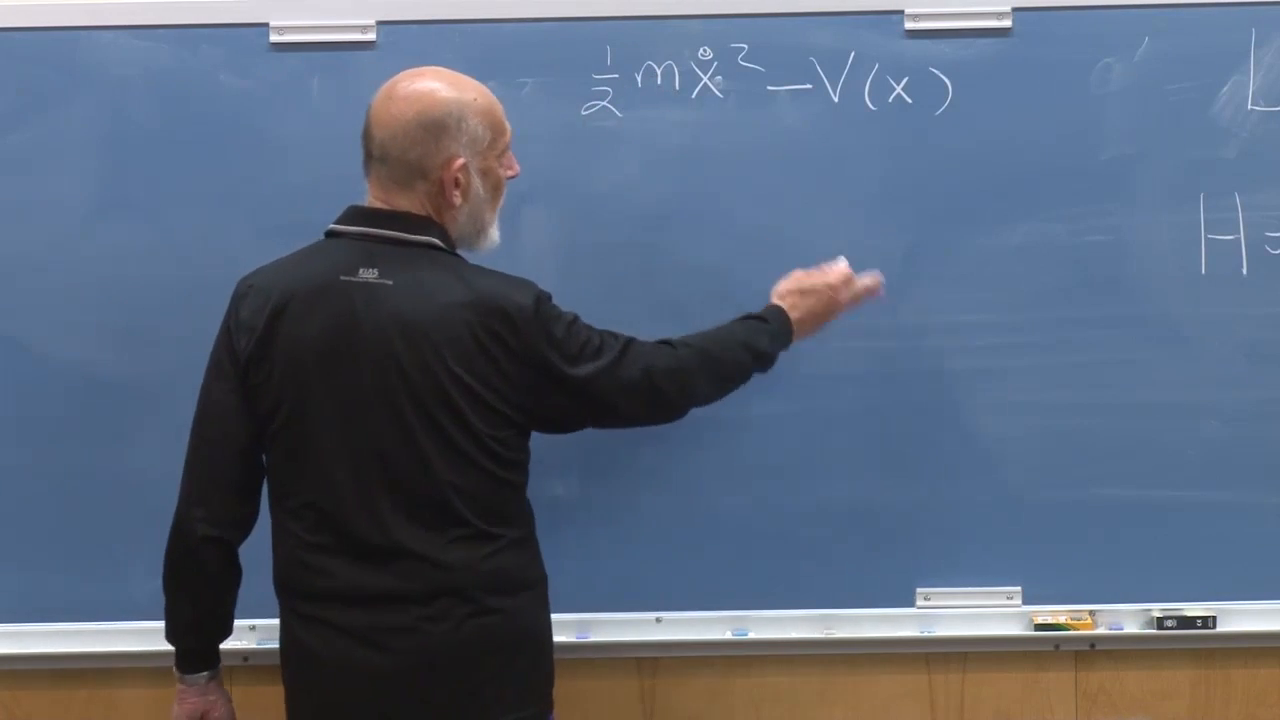
\includegraphics[width=\linewidth]{lecture_10_figure_04.png}
\caption{Член с векторным потенциалом смещает канонический импульс относительно механического.}
\par\smallskip
\textit{Кадр лекции: 00:15:50.}
\end{figure}

\subsection{Нётеровский импульс}

Третий вид импульса — это сохраняющийся заряд, связанный с инвариантностью относительно пространственных переносов. Для бесконечно малого преобразования симметрии
\begin{equation}
q_i\longrightarrow q_i+\delta q_i
\end{equation}
которое оставляет лагранжиан инвариантным, теорема Нётер дает, с точностью до нормировки бесконечно малого параметра,
\begin{equation}
Q=\sum_i p_i\,\delta q_i.
\label{eq:noether-charge-mechanics}
\end{equation}
Появляющиеся здесь \(p_i\) — это канонические импульсы. Если симметрия является однородным переносом и канонический импульс в данном случае совпадает с механическим, \(Q\) сводится к привычному полному импульсу. В менее простой системе такое совпадение нужно доказывать, а не предполагать.

\begin{figure}[H]
\centering
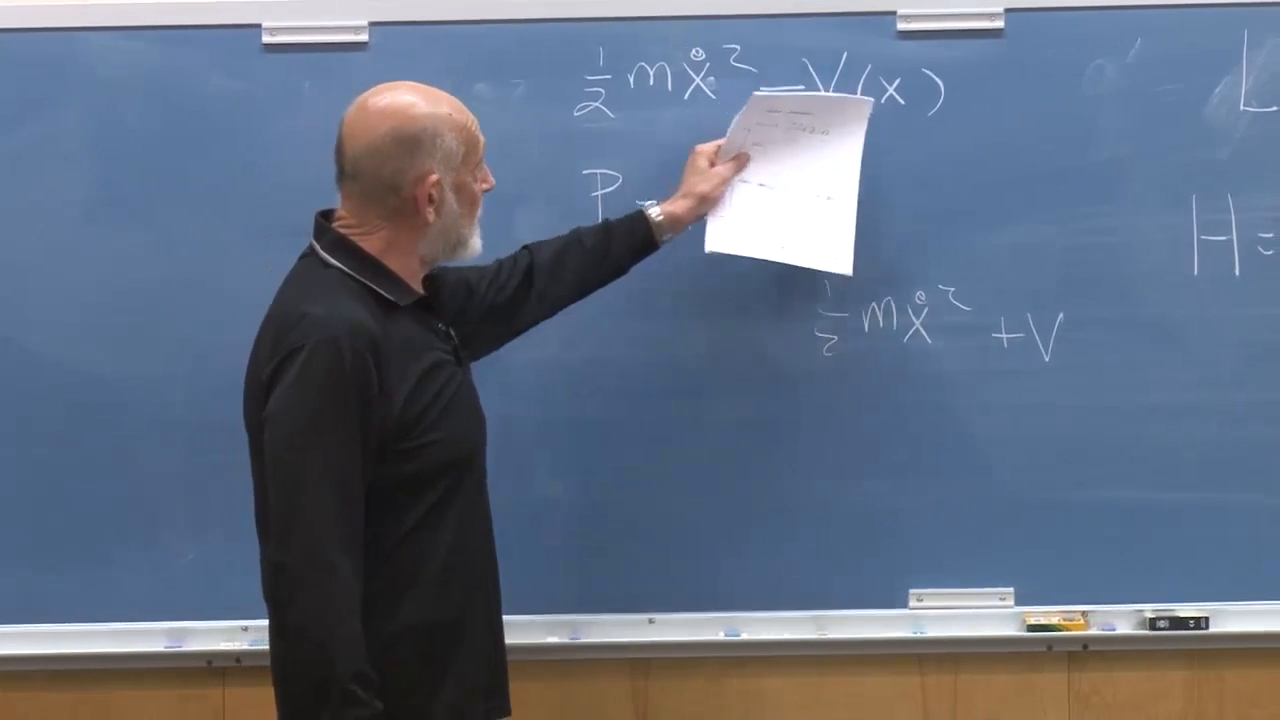
\includegraphics[width=\linewidth]{lecture_10_figure_05.png}
\caption{Заряд Нётер, составленный из канонических импульсов и бесконечно малых изменений координат.}
\par\smallskip
\textit{Кадр лекции: 00:19:00.}
\end{figure}

\section{Энергия как гамильтониан}

Пространственные переносы ведут к импульсу; временные переносы ведут к энергии. Если лагранжиан не зависит явно от времени, гамильтониан
\begin{equation}
H=\sum_i p_i\dot q_i-L
\label{eq:hamiltonian-definition}
\end{equation}
сохраняется. Это преобразование Лежандра лагранжиана, а не правило, позволяющее менять знаки на глаз.

\begin{figure}[H]
\centering
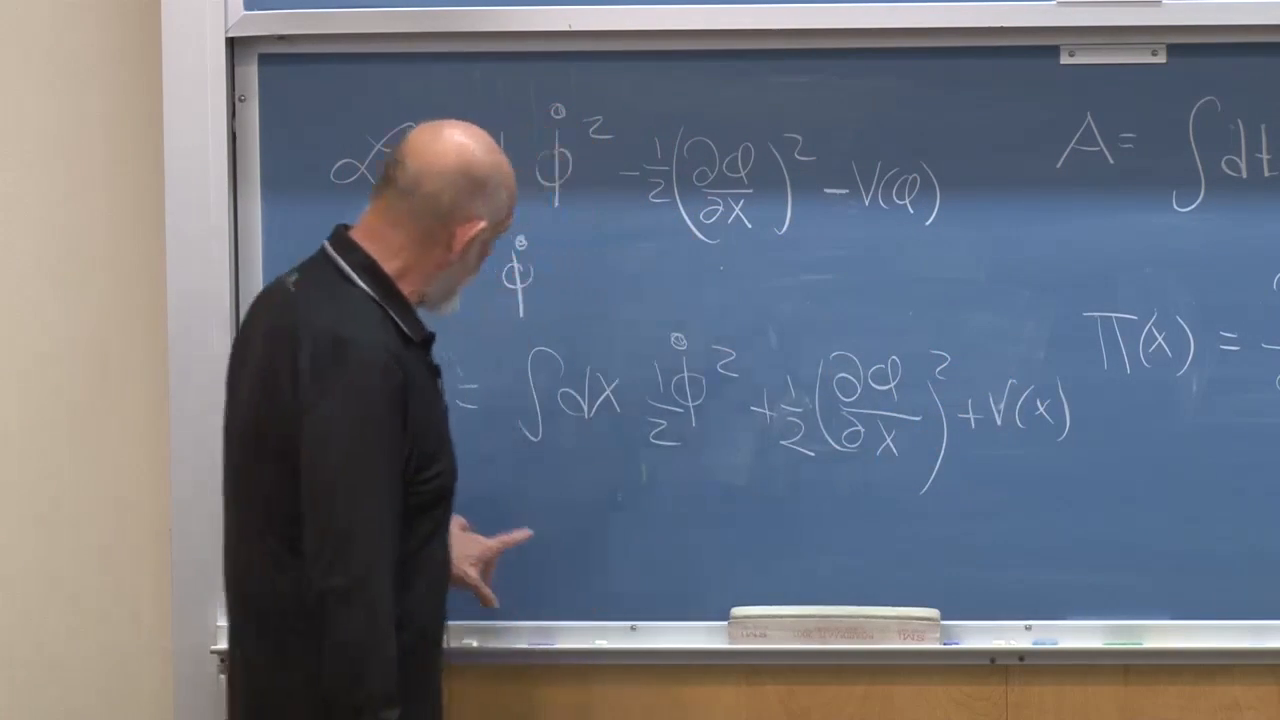
\includegraphics[width=\linewidth]{lecture_10_figure_06.png}
\caption{Гамильтониан, записанный как преобразование Лежандра общего лагранжиана.}
\par\smallskip
\textit{Кадр лекции: 00:22:55.}
\end{figure}

Для примера с одной частицей,
\begin{align}
p&=m\dot x,
\nonumber\\
H&=p\dot x-L\\
&=m\dot x^2
  -\left(\frac12m\dot x^2-V(x)\right)\\
&=\frac12m\dot x^2+V(x).
\label{eq:particle-hamiltonian}
\end{align}
Таким образом, лагранжиан есть кинетическая энергия минус потенциальная, тогда как гамильтониан — кинетическая плюс потенциальная.

\begin{figure}[H]
\centering
\includegraphics[width=\linewidth]{lecture_10_figure_07.png}
\caption{Вычисление для частицы, показывающее, как
\(H=T+V\) следует из \(H=p\dot x-L\).}
\par\smallskip
\textit{Кадр лекции: 00:24:20.}
\end{figure}

Когда вся зависимость от скоростей сводится к обычному положительному квадратичному кинетическому члену, а остальная часть скоростей не содержит, гамильтониан можно получить, изменив знак у части, не зависящей от скоростей. Этим сокращенным приемом мы будем пользоваться неоднократно. Он безопасен только потому, что в рассматриваемых примерах преобразование Лежандра имеет именно такой простой вид.

\section{Поле — это механическая система с континуальным множеством координат}

Чтобы выявить механическую структуру теории поля, выберем одну инерциальную систему отсчета и временно перестанем настаивать на том, чтобы каждая строка явно демонстрировала лоренц-ковариантность. Классическая механика имеет ось времени и координаты \(q_i(t)\). Скалярное поле имеет ось времени и координаты \(\phi(\mathbf x,t)\). Дискретная метка \(i\) просто превратилась в непрерывную метку \(\mathbf x\):
\begin{equation}
q_i(t)\quad\longrightarrow\quad\phi(\mathbf x,t).
\label{eq:discrete-to-field}
\end{equation}
Значение поля в каждой точке пространства составляет одну степень свободы. Здесь \(\mathbf x\) указывает, о какой степени свободы идет речь; само оно не является обобщенной координатой.

\begin{figure}[H]
\centering
\includegraphics[width=\linewidth]{lecture_10_figure_08.png}
\caption{Пространственная решетка, используемая, чтобы представить значение поля в каждой точке как отдельную механическую степень свободы.}
\par\smallskip
\textit{Кадр лекции: 00:30:15.}
\end{figure}

\begin{classroomqa}
\audiencequestion{Почему с самого начала не писать поле как \(\phi(\mathbf x,t)\)?}
\lecturerresponse{Это и есть полное обозначение. Временная запись \(\phi(\mathbf x)\) опускает общий временной аргумент, точно так же как часто пишут \(q_i\), помня, что каждое \(q_i\) зависит от времени. Метка \(i\), а теперь \(\mathbf x\), указывает, о какой степени свободы идет речь. \lecturetimestamp{00:32:43}}
\end{classroomqa}

\begin{classroomqa}
\audiencequestion{Действительно ли значения поля в соседних точках являются независимыми координатами? Что навязывает непрерывность?}
\lecturerresponse{Они являются независимыми каноническими координатами. Гладкость не навязывается отождествлением соседних значений; она отбирается динамикой. Гамильтониан содержит положительный член энергии градиента, поэтому фиксированный скачок на все меньшем расстоянии требует все больше энергии. Следовательно, конфигурации с конечной энергией в пределе континуума являются гладкими. \lecturetimestamp{00:33:09}}
\end{classroomqa}

Пространственная производная делает явной связь между соседними степенями свободы. На решетке с шагом \(\epsilon\),
\begin{equation}
\partial_x\phi(x,t)
  =\lim_{\epsilon\to0}
   \frac{\phi(x+\epsilon,t)-\phi(x,t)}{\epsilon}.
\label{eq:field-finite-difference}
\end{equation}
Она зависит от двух соседних координат, но не содержит обобщенной скорости. В механической аналогии она относится к зависимости лагранжиана от координат, а не к зависимости от \(\dot q_i\).

\begin{figure}[H]
\centering
\includegraphics[width=\linewidth]{lecture_10_figure_09.png}
\caption{Пространственная производная, восстановленная на решетке как разность значений поля в соседних узлах.}
\par\smallskip
\textit{Кадр лекции: 00:31:40.}
\end{figure}

Действие теперь можно записать в явно механической форме:
\begin{align}
S&=\int dt\,L,
\nonumber\\
L&=\int d^3x\,
\mathcal L\!\left(
\phi,\dot\phi,\boldsymbol{\nabla}\phi
\right),
\nonumber\\
S&=\int dt\,d^3x\,
\mathcal L\!\left(
\phi,\dot\phi,\boldsymbol{\nabla}\phi
\right).
\label{eq:field-action-split}
\end{align}
Каллиграфическая буква \(\mathcal L\) обозначает плотность лагранжиана; интегрирование её по пространству даёт обычный лагранжиан, который затем интегрируется по времени. Локальная теория связывает каждую точку только через поля и их производные в этой точке. Отделение времени от пространства на мгновение скрывает лоренц-ковариантность, но делает механику прозрачной.

\begin{figure}[H]
\centering
\includegraphics[width=\linewidth]{lecture_10_figure_10.png}
\caption{Действие поля, разделённое на интеграл по времени и пространственный интеграл от плотности лагранжиана.}
\par\smallskip
\textit{Кадр лекции: 00:36:40.}
\end{figure}

\section{Канонический импульс поля и плотность гамильтониана}

Скорость полевой координаты — это \(\dot\phi(\mathbf x,t)\): скорость изменения поля во времени в одной фиксированной точке. Это не движение из одной пространственной точки в другую. Поэтому канонический импульс, сопряжённый полю, сам является полем,
\begin{equation}
\Pi(\mathbf x,t)
 =\frac{\partial\mathcal L}{\partial\dot\phi(\mathbf x,t)}.
\label{eq:field-canonical-momentum}
\end{equation}
Для нескольких полей \(\phi_a\) каждому соответствует своё поле импульса \(\Pi_a\).

Дискретная сумма в преобразовании Лежандра превращается в пространственный интеграл:
\begin{align}
H
 &=\int d^3x\,
   \left[\Pi\dot\phi-\mathcal L\right]
  =\int d^3x\,\mathcal H,
\nonumber\\
\mathcal H
 &=\Pi\dot\phi-\mathcal L .
\label{eq:field-hamiltonian-density}
\end{align}
Величина под интегралом есть плотность энергии.

\begin{figure}[H]
\centering
\includegraphics[width=\linewidth]{lecture_10_figure_11.png}
\caption{Преобразование Лежандра для поля и его интерпретация как интеграла от локальной плотности энергии.}
\par\smallskip
\textit{Кадр лекции: 00:42:40.}
\end{figure}

\begin{classroomqa}
\audiencequestion{Почему производную полного лагранжиана по \(\dot\phi\) в одной точке можно заменить производной локальной плотности в той же точке?}
\lecturerresponse{Рассматривайте пространственный интеграл как непрерывную сумму.
При использованном здесь предположении локальности скорость \(\dot\phi(\mathbf x)\) входит только в член, принадлежащий этой же точке. Дифференцирование по этой конкретной скорости устраняет все остальные члены. Пространственные производные могут связывать значения поля в соседних точках, но в этой теории они не вводят производных по времени в соседних точках. \lecturetimestamp{00:51:56}}
\end{classroomqa}

\subsection{Скалярное поле}

В одном пространственном измерении возьмём
\begin{equation}
\mathcal L
 =\frac12\dot\phi^2
  -\frac12(\partial_x\phi)^2
  -V(\phi).
\label{eq:scalar-field-lagrangian}
\end{equation}
Это нековариантная запись использованного ранее лоренц-скаляра: относительный знак минус между временными и пространственными производными возникает из метрики Минковского. Канонический импульс равен
\begin{equation}
\Pi=\dot\phi,
\label{eq:scalar-pi}
\end{equation}
а гамильтониан принимает вид
\begin{equation}
H=\int dx\,
\left[
\frac12\dot\phi^2
+\frac12(\partial_x\phi)^2
+V(\phi)
\right].
\label{eq:scalar-field-hamiltonian}
\end{equation}
В ходе вычисления потенциал на мгновение был обозначен как \(V(x)\); аудитория исправила это на \(V(\phi)\). Он может зависеть от положения косвенно, через поле, но в теории, инвариантной относительно трансляций, у него нет заданной внешней зависимости от \(x\).

\begin{figure}[H]
\centering
\includegraphics[width=\linewidth]{lecture_10_figure_12.png}
\caption{Плотность лагранжиана скалярного поля, сопряжённый импульс и положительный гамильтониан, собранные на одной доске.}
\par\smallskip
\textit{Кадр лекции: 00:47:05.}
\end{figure}

Вся часть без производных по времени играет роль потенциальной энергии. Сюда входят как \(V(\phi)\), так и градиентная энергия \(\frac12(\partial_x\phi)^2\). Лагранжиан может иметь любой знак; устойчивая энергия должна быть ограничена снизу.

\begin{classroomqa}
\audiencequestion{Может ли потенциал \(V(\phi)\) быть отрицательным?}
\lecturerresponse{Да. Если у него есть конечная нижняя граница, можно добавить константу так, чтобы его минимум стал равен нулю, не изменяя классического уравнения поля. Потенциал, не ограниченный снизу, описывает неустойчивость: поле может без предела понижать свою энергию. Устойчивый вакуум — это постоянное поле, находящееся в минимуме сдвинутого потенциала.
\lecturetimestamp{00:49:03}}
\end{classroomqa}

Теперь на прежний вопрос о непрерывности дан количественный ответ. Скачок \(\Delta\phi\) на расстоянии между узлами решётки \(\epsilon\) даёт вклад
\begin{equation}
\frac12(\partial_x\phi)^2
\sim\frac12\left(\frac{\Delta\phi}{\epsilon}\right)^2.
\label{eq:gradient-cost}
\end{equation}
При \(\epsilon\to0\) фиксированный скачок даёт сколь угодно большую плотность энергии. Следовательно, конечная энергия подавляет ломаные конфигурации.

\begin{figure}[H]
\centering
\includegraphics[width=\linewidth]{lecture_10_figure_13.png}
\caption{Формула энергии скалярного поля сохранена на доске, а эскиз противопоставляет гладкое поле резкому изменению.}
\par\smallskip
\textit{Кадр лекции: 00:54:20.}
\end{figure}

\section{Локальная энергия и смысл \texorpdfstring{\(T^{00}\)}{T00}}

Плотность энергии получает краткое обозначение:
\begin{equation}
T^{00}=\mathcal H=\Pi\dot\phi-\mathcal L.
\label{eq:T00-definition}
\end{equation}
Два нулевых индекса кодируют два отдельных утверждения. Энергия — это временная компонента \(P^0\) четырёхвектора энергии--импульса, тогда как плотность есть временная компонента сохраняющегося тока. Следовательно, \(T^{00}\) есть плотность временной компоненты четырёхимпульса.

\begin{figure}[H]
\centering
\includegraphics[width=\linewidth]{lecture_10_figure_14.png}
\caption{Энергия поля, записанная локально и отождествлённая с \(T^{00}\).}
\par\smallskip
\textit{Кадр лекции: 01:00:00.}
\end{figure}

Закон сохранения в релятивистской локальной теории — это не просто утверждение о том, что одно глобальное число остаётся неизменным. Энергия не может исчезнуть в лаборатории и появиться вновь на Альфе Центавра. Изменение внутри области должно объясняться потоком через её границу. В локальной форме,
\begin{equation}
\partial_\mu T^{\mu\nu}=0,
\label{eq:stress-energy-continuity}
\end{equation}
поэтому первый индекс обозначает плотность или направление потока, а второй — какую компоненту \(P^\nu\) переносят.

\begin{classroomqa}
\audiencequestion{Означает ли то, что \(T^{00}\) называют плотностью, что полная энергия получается её интегрированием?}
\lecturerresponse{Именно:
\(E=P^0=\int d^3x\,T^{00}\). Локальная плотность — это подынтегральное выражение в полевом преобразовании Лежандра. Её изменение в одном месте компенсируется потоком энергии через соседние участки. \lecturetimestamp{00:59:06}}
\end{classroomqa}

\section{Плотность импульса из пространственных трансляций}

Вернёмся к формуле Нётер, теперь заменив дискретную сумму пространственным интегралом. При малой трансляции в направлении \(m\) поле изменяется на
\begin{equation}
\delta\phi
  =\phi(\mathbf x)-\phi(\mathbf x-\boldsymbol{\epsilon})
  =\epsilon^m\partial_m\phi+O(\epsilon^2),
\label{eq:translated-field-change}
\end{equation}
в пассивной конвенции, использованной на доске. Если поменять местами активные и пассивные трансляции, общий знак меняется на противоположный; физический генератор фиксируется после выбора этой конвенции. Вынося \(\epsilon^m\), получаем, что импульс Нётер имеет вид
\begin{equation}
P_m\ \propto\ \int d^3x\,\Pi\,\partial_m\phi.
\label{eq:scalar-noether-momentum}
\end{equation}

\begin{figure}[H]
\centering
\includegraphics[width=\linewidth]{lecture_10_figure_15.png}
\caption{Сдвинутый профиль поля и производная, измеряющая его бесконечно малое изменение.}
\par\smallskip
\textit{Кадр лекции: 01:04:20.}
\end{figure}

\begin{classroomqa}
\audiencequestion{Почему бесконечно малая трансляция \(\epsilon\) не была сохранена в формуле для импульса?}
\lecturerresponse{Заряд Нётер сначала получается пропорциональным \(\epsilon\). Импульс определяется как коэффициент при этом произвольном параметре трансляции, поэтому результат делят на \(\epsilon\). Умножение сохраняющейся величины на фиксированную константу не повлияло бы на её сохранение, но выделение коэффициента даёт стандартную нормировку.
\lecturetimestamp{01:04:45}}
\end{classroomqa}

\begin{classroomqa}
\audiencequestion{Переходит ли интервал трансляции в \(dx\) в континуальном интеграле?}
\lecturerresponse{Они возникают из разных предельных переходов. Мера \(dx\) появляется при замене суммы по пространственно помеченным степеням свободы интегралом. Параметр трансляции \(\epsilon\) описывает операцию симметрии и выносится из соответствующего заряда Нётер. Оба бесконечно малы в промежуточных рассуждениях, но играют разные роли.
\lecturetimestamp{01:05:16}}
\end{classroomqa}

В обозначениях лекции плотность \(m\)-й компоненты импульса равна
\begin{equation}
T^{0m}=\Pi\,\partial_m\phi,
\label{eq:scalar-momentum-density}
\end{equation}
с подразумеваемой конвенцией знака трансляции. Для скалярной теории \(\Pi=\dot\phi\), так что она пропорциональна
\(\dot\phi\,\partial_m\phi\).

\begin{figure}[H]
\centering
\includegraphics[width=\linewidth]{lecture_10_figure_16.png}
\caption{Плотность импульса Нётер
\(T^{0m}=\Pi\,\partial_m\phi\) на доске.}
\par\smallskip
\textit{Кадр лекции: 01:07:10.}
\end{figure}

Это буквально импульс, переносимый волной. Инвариантность относительно трансляций действует только тогда, когда сдвигается всё: поля, частицы, источники и аппаратура. Световой импульс, поглощённый свободно подвешенной пластинкой, сообщает ей отдачу. Для обычного света эффект крошечный; достаточно мощный лазер может передать достаточно импульса, чтобы сжать небольшую мишень. Сохраняющаяся полная величина принадлежит совместно частицам и полям.

\subsection{Что заменяет уравнение Ньютона?}

Уравнение Эйлера--Лагранжа для поля, выведенное из уравнения~\eqref{eq:scalar-field-lagrangian}, имеет вид
\begin{equation}
\ddot\phi-\nabla^2\phi=-\frac{dV}{d\phi}.
\label{eq:scalar-equation-of-motion}
\end{equation}
Это полевой аналог закона Ньютона.

\begin{figure}[H]
\centering
\includegraphics[width=\linewidth]{lecture_10_figure_17.png}
\caption{Уравнение скалярного поля, выписанное рядом с его гамильтонианом и плотностью импульса.}
\par\smallskip
\textit{Кадр лекции: 01:12:55.}
\end{figure}

\begin{classroomqa}
\audiencequestion{Что соответствует закону Ньютона для поля?}
\lecturerresponse{Эту роль играет уравнение поля Эйлера--Лагранжа. Здесь это волновое уравнение с силовым членом \(-V'(\phi)\). Роль \(m\ddot x=-V'(x)\) играет
\(\ddot\phi-\nabla^2\phi=-V'(\phi)\).
\lecturetimestamp{01:11:48}}
\end{classroomqa}

\begin{classroomqa}
\audiencequestion{Как узнать, что предложенный лагранжиан поля корректен? Должны ли мы уже знать уравнение поля?}
\lecturerresponse{Возможны оба направления. Исторически можно вывести уравнения из эксперимента, а затем искать действие, как было у Newton и Maxwell. В современной теории часто начинают с набора полей, локальности, симметрии и небольшого набора допустимых членов, выводят уравнения и проверяют их предсказания. Приведённое скалярное поле может описывать фундаментальное поле, но с тем же успехом может описывать поперечное смещение верёвки, чьё континуальное действие выводится из составляющих её частиц. \lecturetimestamp{01:12:55}}
\end{classroomqa}

\section{Электромагнитное поле во временной калибровке}

Уже найденные компоненты, \(T^{00}\) и \(T^{0m}\), принадлежат тензору энергии--импульса. Остальные его компоненты описывают потоки энергии и импульса. Позднее этот тензор будет источником гравитации, но непосредственный пример даёт электромагнетизм.

Базовой электромагнитной координатой служит четырёхпотенциал \(A_\mu\).
Калибровочная свобода допускает
\begin{equation}
A_\mu\longrightarrow A'_\mu=A_\mu+\partial_\mu S
\label{eq:gauge-transformation-lecture10}
\end{equation}
без изменения \(F_{\mu\nu}\). Выберем \(S\) так, чтобы выполнялось
\begin{equation}
\partial_tS=-A_0.
\label{eq:temporal-gauge-choice}
\end{equation}
Например, в каждой фиксированной пространственной точке можно проинтегрировать \(A_0\) по времени. Тогда преобразованная временная компонента обращается в нуль:
\begin{equation}
A'_0=A_0+\partial_tS=0.
\label{eq:temporal-gauge}
\end{equation}
Это временная калибровка. Она исключает \(A_0\) из списка динамических координат, хотя закон Гаусса остаётся связью и сохраняется остаточная калибровочная свобода, не зависящая от времени.

\begin{figure}[H]
\centering
\includegraphics[width=\linewidth]{lecture_10_figure_18.png}
\caption{Калибровочная свобода используется для выбора \(A_0=0\) путём решения \(\partial_tS=-A_0\).}
\par\smallskip
\textit{Кадр лекции: 01:20:15.}
\end{figure}

Начиная с этого места, пусть \(\mathbf E\) обозначает стандартное электрическое поле Максвелла. Перед фиксацией калибровки,
\begin{equation}
E_m=-\partial_tA_m+\partial_mA_0,
\qquad
\mathbf B=\boldsymbol{\nabla}\times\mathbf A.
\label{eq:E-B-general-potential}
\end{equation}
Во временной калибровке это сводится к
\begin{equation}
\mathbf E=-\dot{\mathbf A},
\qquad
\mathbf B=\boldsymbol{\nabla}\times\mathbf A.
\label{eq:E-B-temporal-gauge}
\end{equation}
Производные по времени от \(\mathbf A\) дают электрическое поле; пространственные производные дают магнитное поле.

\begin{figure}[H]
\centering
\includegraphics[width=\linewidth]{lecture_10_figure_19.png}
\caption{Электрическое и магнитное поля во временной калибровке:
\(\mathbf E=-\dot{\mathbf A}\) и
\(\mathbf B=\nabla\times\mathbf A\).}
\par\smallskip
\textit{Кадр лекции: 01:23:50.}
\end{figure}

\section{Канонический импульс и энергия электромагнитного поля}

Плотность лагранжиана свободного поля Максвелла равна
\begin{equation}
\mathcal L_{\mathrm{EM}}
 =-\frac14F_{\mu\nu}F^{\mu\nu}
 =\frac12\left(\mathbf E^2-\mathbf B^2\right).
\label{eq:maxwell-lagrangian-energy-lecture}
\end{equation}
Во временной калибровке,
\begin{equation}
\mathcal L_{\mathrm{EM}}
 =\frac12\dot{\mathbf A}^{\,2}
  -\frac12(\boldsymbol{\nabla}\times\mathbf A)^2.
\label{eq:maxwell-lagrangian-temporal}
\end{equation}
Она имеет в точности ту же структуру, что и для скалярного поля: квадраты производных по времени минус квадраты пространственных производных.

\begin{figure}[H]
\centering
\includegraphics[width=\linewidth]{lecture_10_figure_20.png}
\caption{Лагранжиан Максвелла, переписанный как механический лагранжиан поля для пространственных компонент \(\mathbf A\).}
\par\smallskip
\textit{Кадр лекции: 01:28:10.}
\end{figure}

У каждой компоненты \(A_m\) есть канонический импульс,
\begin{equation}
\Pi_m
 =\frac{\partial\mathcal L_{\mathrm{EM}}}
        {\partial\dot A_m}
 =\dot A_m
 =-E_m.
\label{eq:em-canonical-momentum}
\end{equation}
Это наглядный пример того, почему соглашение имеет значение. При использовавшемся ранее противоположном соглашении для электрического поля последний выписанный знак изменился бы, хотя сама каноническая производная не изменилась бы.

\begin{figure}[H]
\centering
\includegraphics[width=\linewidth]{lecture_10_figure_21.png}
\caption{Три поля канонического импульса, связанные с
\(A_x,A_y,A_z\); каждое равно соответствующей производной по времени и,
следовательно, минус стандартному электрическому полю.}
\par\smallskip
\textit{Кадр лекции: 01:30:20.}
\end{figure}

Теперь оправдан гамильтонов быстрый приём: надо поменять знак у члена без производной по времени. Плотность энергии электромагнитного поля равна
\begin{equation}
T^{00}_{\mathrm{EM}}
 =\mathcal H_{\mathrm{EM}}
 =\frac12\left(\mathbf E^2+\mathbf B^2\right),
\label{eq:em-energy-density}
\end{equation}
а полная энергия равна
\begin{equation}
H_{\mathrm{EM}}
 =\int d^3x\,
\frac12\left(\mathbf E^2+\mathbf B^2\right).
\label{eq:em-total-energy}
\end{equation}
В отличие от плотности лагранжиана, плотность энергии неотрицательна.

\begin{figure}[H]
\centering
\includegraphics[width=\linewidth]{lecture_10_figure_22.png}
\caption{Положительная гамильтонова плотность электромагнитного поля
\(\frac12(\mathbf E^2+\mathbf B^2)\).}
\par\smallskip
\textit{Кадр лекции: 01:32:00.}
\end{figure}

Для плоской волны в вакууме, \(\mathbf E\perp\mathbf B\), эти два поля синфазны, и в единицах \(c=1\) их модули равны. Поэтому электрический и магнитный вклады поровну делят энергию волны:
\begin{equation}
u_E=\frac12\mathbf E^2,
\qquad
u_B=\frac12\mathbf B^2,
\qquad
u_E=u_B.
\label{eq:plane-wave-energy-halves}
\end{equation}

\section{Вывод электромагнитного импульса}

Формулу Нётер для трансляций теперь нужно просуммировать по трём полям \(A_m\). Если знак трансляции выбран так, чтобы физический импульс был направлен вдоль распространения волны, то \(n\)-я компонента равна
\begin{equation}
P_n
 =\int d^3x\,E_m\,\partial_nA_m,
\label{eq:em-canonical-noether-momentum}
\end{equation}
где подразумевается суммирование по \(m\). В лекции на этом знаке намеренно задерживаются: он зависит от сделанных ранее выборов соглашения для электрического поля и активной/пассивной трансляции. Калибровочно-инвариантный физический результат его зафиксирует.

\begin{figure}[H]
\centering
\includegraphics[width=\linewidth]{lecture_10_figure_23.png}
\caption{Формула Нётер для скалярного поля, распространённая на три
компоненты векторного потенциала.}
\par\smallskip
\textit{Кадр лекции: 01:36:40.}
\end{figure}

Подынтегральное выражение всё ещё содержит калибровочный потенциал, а не только физические поля. Прибавим и вычтем
\(E_m\partial_mA_n\):
\begin{align}
E_m\partial_nA_m
 &=
 E_m\left(\partial_nA_m-\partial_mA_n\right)
 +E_m\partial_mA_n.
\label{eq:add-subtract-em-momentum}
\end{align}
Первый член есть векторное произведение,
\begin{equation}
E_m\left(\partial_nA_m-\partial_mA_n\right)
  =(\mathbf E\times\mathbf B)_n.
\label{eq:cross-product-component}
\end{equation}
Второй член интегрируется по частям:
\begin{align}
\int d^3x\,E_m\partial_mA_n
 &=
\int_{\partial V}d\Sigma_m\,E_mA_n
-\int d^3x\,A_n\partial_mE_m.
\label{eq:em-momentum-integration-parts}
\end{align}
Если поля убывают так, что граничный член исчезает, и если область свободна от источников, так что
\(\boldsymbol{\nabla}\cdot\mathbf E=0\), то второй член не даёт вклада.

\begin{figure}[H]
\centering
\includegraphics[width=\linewidth]{lecture_10_figure_24.png}
\caption{Добавленный член, перенесённый интегрированием по частям к
\(\nabla\cdot\mathbf E\).}
\par\smallskip
\textit{Кадр лекции: 01:40:00.}
\end{figure}

Следовательно, полный импульс поля равен
\begin{equation}
\mathbf P_{\mathrm{EM}}
 =\int d^3x\,\mathbf E\times\mathbf B,
\qquad
\mathbf g_{\mathrm{EM}}
 =\mathbf E\times\mathbf B,
\label{eq:em-momentum-density}
\end{equation}
в единицах, принятых в лекции. Вектор
\(\mathbf g_{\mathrm{EM}}\) есть плотность электромагнитного импульса.

\begin{figure}[H]
\centering
\includegraphics[width=\linewidth]{lecture_10_figure_25.png}
\caption{Выражение через калибровочный потенциал, сведённое к
калибровочно-инвариантному импульсу \(\int d^3x\,\mathbf E\times\mathbf B\).}
\par\smallskip
\textit{Кадр лекции: 01:41:10.}
\end{figure}

\begin{classroomqa}
\audiencequestion{Где использовалось
\(\boldsymbol{\nabla}\cdot\mathbf E=0\), и что происходит при наличии зарядов?}
\lecturerresponse{Оно устраняет объёмный член после интегрирования по
частям, так что приведённый вывод только через поля применим к свободной
электромагнитной волне. При наличии заряда этот член не равен нулю, и
нужно включить импульс заряженного вещества. Инвариантность
относительно трансляций и сохранение импульса относятся к полной
системе вещество--поле. \lecturetimestamp{01:41:55}}
\end{classroomqa}

\subsection{Направление импульса волны}

В плоской волне \(\mathbf E\), \(\mathbf B\) и направление
распространения образуют правую тройку. Через полдлины волны и
\(\mathbf E\), и \(\mathbf B\) меняют знак:
\begin{equation}
(-\mathbf E)\times(-\mathbf B)
 =\mathbf E\times\mathbf B.
\label{eq:poynting-sign-reversal}
\end{equation}
Поэтому плотность импульса на всём протяжении колебания направлена в
одну и ту же фиксированную сторону — в сторону распространения волны.

\begin{figure}[H]
\centering
\includegraphics[width=\linewidth]{lecture_10_figure_26.png}
\caption{Геометрия плоской волны: электрическое и магнитное поля меняют знак
одновременно, а их векторное произведение по-прежнему направлено вдоль оси
распространения.}
\par\smallskip
\textit{Кадр лекции: 01:43:10.}
\end{figure}

Вот почему давление света реально. При поглощении импульс поля
передаётся веществу; при отражении импульс света меняет направление и может
передать отражателю удвоенную нормальную компоненту.

\section{Где потенциал соприкасается с наблюдаемыми полями}

В конце занятия аудитория спрашивает о точках соприкосновения между
\(A_\mu\) и наблюдаемыми полями. Это в точности
\begin{align}
E_n&=-\partial_tA_n+\partial_nA_0,
\nonumber\\
B_n&=\epsilon_{nmk}\partial_mA_k.
\label{eq:potential-field-contact}
\end{align}
Временная калибровка убирает член с \(A_0\), но не изменяет физические
поля.

\begin{figure}[H]
\centering
\includegraphics[width=\linewidth]{lecture_10_figure_27.png}
\caption{Общее соотношение для электрического поля, восстановленное после
вычисления во временной калибровке, вместе с ковариантным скалярным
лагранжианом, напомненным под ним.}
\par\smallskip
\textit{Кадр лекции: 01:45:40.}
\end{figure}

\begin{classroomqa}
\audiencequestion{Где именно связываются векторный потенциал и
электрическое и магнитное поля?}
\lecturerresponse{Электрическое поле сочетает производную по времени от
пространственного потенциала с пространственной производной \(A_0\); магнитное
поле есть ротор пространственного потенциала. Во временной калибровке
это просто сводится к
\(\mathbf E=-\dot{\mathbf A}\) и
\(\mathbf B=\nabla\times\mathbf A\).
\lecturetimestamp{01:44:15}}
\end{classroomqa}

\begin{classroomqa}
\audiencequestion{Является ли потенциал более фундаментальным, чем
\(\mathbf E\) и \(\mathbf B\)?}
\lecturerresponse{Действие и калибровочный принцип естественнее всего
формулируются через \(A_\mu\), что делает потенциал структурно
более фундаментальным. Однако \(A_\mu\) не единственен: потенциалы,
связанные калибровочным преобразованием, представляют одну и ту же физику, а
локальные поля калибровочно инвариантны. Эти два утверждения совместимы.
Фундаментальные переменные не обязаны сами по себе быть непосредственно
наблюдаемыми. \lecturetimestamp{01:46:36}}
\end{classroomqa}

\begin{classroomqa}
\audiencequestion{Может ли сам калибровочный потенциал оказывать силу?}
\lecturerresponse{Калибровочно-зависимый представитель не может порождать
калибровочно-зависимую измеримую силу. Заряженное вещество связано с
потенциалом через действие, но классическую силу Лоренца можно целиком
записать через калибровочно-инвариантные электрическое и магнитное поля.
\lecturetimestamp{01:47:49}}
\end{classroomqa}

\begin{classroomqa}
\audiencequestion{Если скрещенные электрическое и магнитное поля стационарны, должен ли их импульс быть нулевым?}
\lecturerresponse{Не обязательно для самого поля: \(\mathbf E\times\mathbf B\) может быть ненулевым даже тогда, когда оба поля не зависят от времени. В замкнутой статической установке полный баланс импульса включает также заряды, токи, опоры и любой механический или скрытый импульс. Краткий ответ в аудитории о том, что полный баланс должен уравновешиваться, и есть правильная формулировка закона сохранения; приравнивать к нулю один лишь вклад поля было бы слишком сильным требованием.
\lecturetimestamp{01:48:01}}
\end{classroomqa}

\section{Один тензор, два смысла вектора Пойнтинга}

Тензор энергии--импульса объединяет все плотности и потоки:
\begin{align}
T^{00}&=\text{energy density},\\
T^{0i}&=\text{\(i\)-momentum density},\\
T^{i0}&=\text{energy flux in the \(i\)-direction},\\
T^{ij}&=\text{\(j\)-momentum flux in the \(i\)-direction}.
\label{eq:stress-energy-components}
\end{align}
Например, \(T^{31}\) — это количество \(x\)-импульса, проходящего за единицу времени через единичную площадку с нормалью в \(z\)-направлении. Пространственный блок \(T^{ij}\) — это тензор напряжений.

\begin{figure}[H]
\centering
\includegraphics[width=\linewidth]{lecture_10_figure_28.png}
\caption{На доске начинают собирать компоненты плотности и потока в тензор энергии--импульса.}
\par\smallskip
\textit{Кадр лекции: 01:51:10.}
\end{figure}

Для обсуждаемых релятивистских систем физический тензор энергии--импульса можно выбрать симметричным:
\begin{equation}
T^{\mu\nu}=T^{\nu\mu}.
\label{eq:stress-energy-symmetry}
\end{equation}
Следовательно,
\begin{equation}
T^{0i}=T^{i0}.
\label{eq:momentum-density-energy-flux}
\end{equation}
Плотность \(i\)-импульса равна потоку энергии в \(i\)-направлении при \(c=1\). Это и есть ответ на последний вопрос из аудитории: вектор Пойнтинга действительно является плотностью мощности.

\begin{classroomqa}
\audiencequestion{Является ли \(\mathbf E\times\mathbf B\) плотностью мощности, а не плотностью импульса?}
\lecturerresponse{И тем и другим. Симметрия \(T^{\mu\nu}\) отождествляет плотность импульса \(T^{0i}\) с потоком энергии \(T^{i0}\). Тем самым \(\mathbf S=\mathbf E\times\mathbf B\) — это энергия в единицу времени на единицу площади и, в единицах \(c=1\), импульс на единицу объёма. После восстановления обычных единиц получается \(\mathbf g=\mathbf S/c^2\).
\lecturetimestamp{01:48:20}}
\end{classroomqa}

\begin{figure}[H]
\centering
\includegraphics[width=\linewidth]{lecture_10_figure_29.png}
\caption{Симметричное тензорное соотношение, приравнивающее плотность импульса потоку энергии и обозначенное на доске вектором Пойнтинга.}
\par\smallskip
\textit{Кадр лекции: 01:53:50.}
\end{figure}

\section{Мост к общей теории относительности}

Курс завершается тем, что классическая механика, теория поля и электромагнетизм сводятся в единую структуру:
\begin{enumerate}
\item Инвариантность относительно сдвигов по времени даёт гамильтониан и энергию.
\item Инвариантность относительно пространственных сдвигов даёт нётеровский импульс.
\item Замена дискретных координат полями, зависящими от пространственной координаты, превращает суммы в интегралы, а сохраняющиеся величины — в локальные плотности.
\item Фиксация калибровки выявляет механические координаты поля Максвелла, не изменяя его наблюдаемых величин.
\item Гамильтониан Максвелла даёт
\(\frac12(\mathbf E^2+\mathbf B^2)\), тогда как пространственные сдвиги дают
\(\mathbf E\times\mathbf B\).
\item Симметричный тензор энергии--импульса объединяет плотность энергии, плотность импульса, поток энергии и напряжения.
\end{enumerate}

Именно эта величина понадобится на следующем этапе. В общей теории относительности тензор энергии--импульса выступает источником в уравнении поля Эйнштейна. Поэтому заключительная лекция не просто добавила электромагнитное вычисление; она подготовила язык, на котором материя и поля сообщают пространству-времени, как ему искривляться.